\section{Planung der Implementierungsphase}

Die Implementierungsphase lässt sich grob in sechs Phasen (Vorbereitung, Parser, Interpreter, Beweiserschnittstelle, GUI, Dokumentation) einteilen. Die ungefähre Zeitplanung und die Abhängigkeiten jedes Arbeitsschrittes sind in Abbildung~\ref{gantt_impl} verdeutlicht. Die geschätzten Zeiten werden in Tabelle~\ref{timeplan} dargestellt.

\begin{figure}
	\centering
	\hspace*{-2cm}\vspace*{-2cm}\caption[B]{Die Tasks der Implementierungsphase und ihre Abhängigkeiten}
	\hspace*{-3cm}\vspace*{-3cm}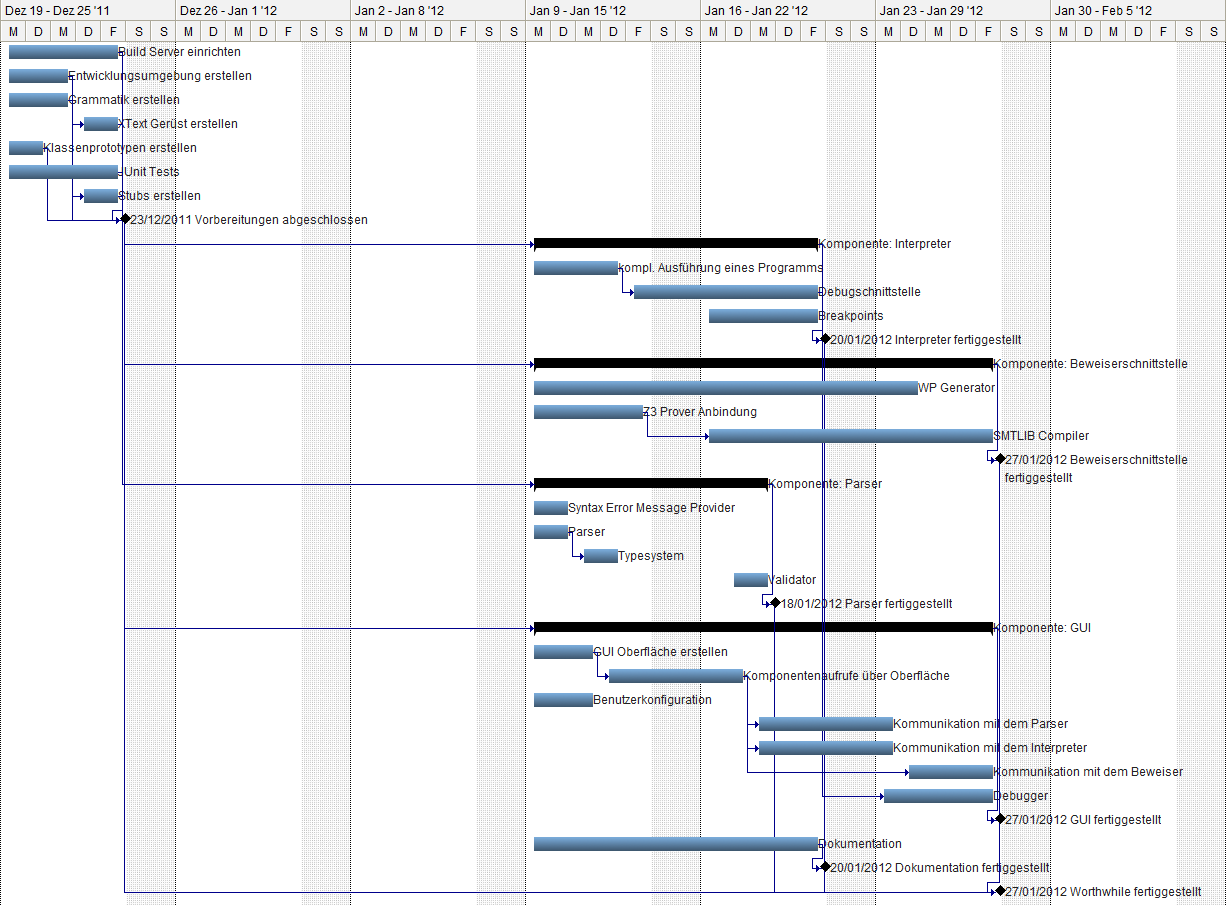
\includegraphics[angle=90,width=19cm,height= 25cm]{diagrams/gantt_implementierung_diag.png}
	\label{gantt_impl}
\end{figure}

\begin{table}[H]
	\caption[B]{Ungefähre Zeiteinteilung (in Stunden) für die Implementierungsphase}
	\label{timeplan}
	\begin{tabular}{|l|l|l|l|l|l|l|}
		\hline
		 & \textbf{Leon} & \textbf{Chris} & \textbf{Stefan} & \textbf{Joachim} & \textbf{Fabian} & \textbf{Matthias} \\
		\hline
		\textbf{Vorbereitungen} & 12 & 12 & 12 & 12 & 12 & 12 \\
		\hline
		\textbf{Interpreter} & 34 & 0 & 0 & 0 & 0 & 19 \\
		\hline
		\textbf{Beweiserschnittstelle} & 14 & 8 & 24 & 0 & 48 & 0 \\
		\hline
		\textbf{Parser} & 0 & 0 & 11 & 0 & 0 & 17 \\
		\hline
		\textbf{GUI} & 0 & 22 & 13 & 48 & 0 & 12 \\
		\hline
		\textbf{Dokumentation} & 3 & 19 & 3 & 3 & 3 & 3 \\
		\hline
		\textbf{Gesamt}	& 63 & 61 & 63 & 63 & 63 & 63 \\
		\hline
	\end{tabular}
\end{table}

\subsection{Vorbereitungen}
In der Vorbereitungsphase, welche allen anderen Phasen voranliegt, wird hauptsächlich das Klassendiagramm in Quelltext umgesetzt sowie eine Basis für die Implementierungen eingerichtet. Hierzu gehört insbesondere das Erstellen der Grammatik für die WHILE-Sprache und das Ausrüsten aller Komponenten mit Stubs, um eingeschränkt funktionierende Schnittstellen für die anderen Teile des Programms bereitzustellen. Desweiteren werden JUnit-""Tests erstellt, die implementierungsbegleitend benutzt werden sollen. Durch die vorgesehenen Stubs müssen alle JUnit-""Tests erfolgreich ausgeführt werden. Im späteren Verlauf der Implementierungsphase wird Wert darauf gelegt, dass ein Stub nur dann gegen eine funktionierende Schnittstelle ausgetauscht wird, wenn gewährleistet ist, dass der zuständige JUnit-""Test immer noch erfolgreich abläuft. Für diese Phase werden alle Mitglieder des Teams in etwa gleich beansprucht. Nach erfolgreicher Beendigung der Vorbereitungen können die Phasen für die jeweiligen Komponenten des Projekts (Interpreter mit Run-""time-""Checker, Beweiserschnittstelle, GUI) anlaufen.

\subsection{Parser}
Möglichst frühzeitig wird die Parserfunktionalität soweit erstellt, dass das Parsen eines Programms möglich ist. Dieser Teil ist von hoher Wichtigkeit, da hierdurch das übrige Projekt auf einen eigens erstellten Abstract-""Syntax-""Tree (jedoch ohne semantische Prüfung) zurückgreifen kann und nicht mehr abhängig von der Ausgabe des Stubs ist.

% TODO Syntax Error Message Provider?

Anschließend kann die Einbindung des Typsystems erfolgen und die Funktionalität des Validators aufgenommen werden.

\subsection{Interpreter}
Zu Beginn dieser Phase erfolgt die Implementierung der Grundfunktionalität des Interpreters. Die komplette Ausführung eines ASTs soll ermöglicht werden, um Fehler des vom Parser erzeugten Abstract-""Syntax-""Trees frühzeitig zu erkennen. Einen hohen Stellenwert bekommt die Debugschnittstelle, welche direkt nach Implementierung der Grundfunktionalität entwickelt wird. Die Einbindung der Unterstützung für Breakpoints kann parallel hierzu erfolgen.

\subsection{Beweiserschnittstelle}
In dieser Phase ist der Teil für die Generierung der Weakest-""Precondition unabhängig von der Anbindung des Beweisers und des Compilers für die SMTLIB-Sprache und kann somit parallel hierzu bearbeitet werden. Die Übersetzung von Formeln in SMTLIB ist abhängig von der Anbindung des Beweisers, da es hiermit ermöglicht wird, den SMTLIB-Compiler zu testen und damit auch korrekt zu implementieren.

\subsection{GUI}
Die GUI kann in vielen Bereichen unabhängig vom Rest des Projekts entwickelt werden. Es ist jedoch von Vorteil die Kommunikation mit den einzelnen Komponenten erst dann zu implementieren, wenn eine gewisse Grundfunktionalität der jeweiligen Komponente gegeben ist. Deshalb wird die Oberfläche der GUI zu Beginn erstellt und anschließend die Aufrufe von der Oberfläche zu den Kommunikationsschnittstellen integriert. Gleichzeitig kann mit der Implementierung des Teils der Benutzerkonfiguration erfolgen. Erst dann wird mit der Implementierung der Kommunikationskomponenten begonnen. Der Debugger wird entwickelt, sobald der Interpreter fertiggestellt ist.

\subsection{Dokumentation}
Die Dokumentation besteht aus einem ausführlichen Benutzerhandbuch, einer Schnittstellendokumentation sowie Beispielprogrammen. Sie wird begleitend mit allen Phasen erstellt und sichert Konsistenz und Vollständigkeit. Desweiteren ist es hilfreich diese eher zu Beginn zu entwickeln, da dies wiederum die Implementierung unterstützt. Bei dieser Phase wird jedes Teammitglied, überwiegend in seinem zugehörigen Bereich, beteiligt sein.
